\documentclass[a4paper,12pt]{article}

\usepackage[T2A]{fontenc}			
\usepackage[utf8]{inputenc}			
\usepackage[english,russian]{babel}	

\usepackage[
bookmarks=true, colorlinks=true, unicode=true,
urlcolor=black,linkcolor=black, anchorcolor=black,
citecolor=black, menucolor=black, filecolor=black,
]{hyperref}

\usepackage{color}
\usepackage{caption}
\DeclareCaptionFont{white}{\color{black}}
\DeclareCaptionFormat{listing}{\colorbox{white}{\parbox{\textwidth}{#1#2#3}}}
\captionsetup[lstlisting]{format=listing,labelfont=white,textfont=white}

\usepackage{amsmath,amsfonts,amssymb,amsthm,mathtools} 
\usepackage{wasysym}

\usepackage{graphicx}
%\usepackage[cache=false]{minted}
\usepackage{cmap}
\usepackage{indentfirst}

\usepackage{listings} 
\usepackage{fancyvrb}

\usepackage{geometry}
\geometry{left=2cm}
\geometry{right=1.5cm}
\geometry{top=1cm}
\geometry{bottom=2cm}

\setlength{\parindent}{5ex}
\setlength{\parskip}{0.5em}

\usepackage{pgfplots}
\usetikzlibrary{datavisualization}
\usetikzlibrary{datavisualization.formats.functions}

\begin{document}
	\lstset{ %
		language=C,                 % выбор языка для подсветки (здесь это С)
		basicstyle=\small\sffamily, % размер и начертание шрифта для подсветки кода
		numbers=left,               % где поставить нумерацию строк (слева\справа)
		numberstyle=\tiny,           % размер шрифта для номеров строк
		stepnumber=1,                   % размер шага между двумя номерами строк
		numbersep=5pt,                % как далеко отстоят номера строк от подсвечиваемого кода
		backgroundcolor=\color{white}, % цвет фона подсветки - используем \usepackage{color}
		showspaces=false,            % показывать или нет пробелы специальными отступами
		showstringspaces=false,      % показывать или нет пробелы в строках
		showtabs=false,             % показывать или нет табуляцию в строках
		frame=single,              % рисовать рамку вокруг кода
		tabsize=2,                 % размер табуляции по умолчанию равен 2 пробелам
		captionpos=t,              % позиция заголовка вверху [t] или внизу [b] 
		breaklines=true,           % автоматически переносить строки (да\нет)
		breakatwhitespace=false, % переносить строки только если есть пробел
		escapeinside={\%*}{*)}   % если нужно добавить комментарии в коде
	}
	
	% Титульный лист
	\large
	\begin{center}
		Федеральное государственное бюджетное образовательное учреждение 
		высшего образования <<Московский государственный технический 
		университет имени Н. Э. Баумана>> 
		(национальный исследовательский университет)
	\end{center}
	
	\vspace*{30mm} 
	
	\huge
	\begin{center}
		Дисциплина: <<Анализ алгоритмов>>
		
		Отчет по рубежному контролю №1
	\end{center}
	
	\vspace*{30mm} 
	
	\huge
	\begin{center}
		Тема работы:\\
		<<Дерево Пифагора>>
	\end{center}
	\vspace*{30mm} 
	
	\large
	\begin{flushright}
		Студент: Левушкин И. К. \\
		Группа: ИУ7-52Б \\
		Преподаватели: Волкова Л. Л., \\ Строганов Ю. В. \\
	\end{flushright}
	
	\vspace*{40mm}
	\begin{center}
		Москва, 2019 г.  
	\end{center}
	\thispagestyle{empty}
	
	\tableofcontents
	
	\section*{Введение}
	\addcontentsline{toc}{section}{Введение}
	
	\textbf{Цель лабораторной работы:} При помощи конечных автоматов и регулярных выражений написать программу, находящую группы факультетов ИУ, ИБМ и Э в тексте.
	
	\textbf{Задачи работы:}
	
	\begin{enumerate} 
		\item[1)] изучить работу регулярных выражений и конечных автоматов;
		\item[2)] создать конечный автомат;
		\item[3)] реализовать поставленную задачу с использованием конечного автомата;
		\item[4)] реализовать поставленную задачу с использованием регулярные выражения;
		\item[5)] сравнить время выполнения программы, использующую конечный автомат, и программу, использующую регулярные выражения;
		\item[6)] описать и обосновать полученные результаты в отчете о рубежном контроле 
		работе, выполненного как расчётно-пояснительная записка. 
	\end{enumerate} 
	\pagebreak
	
	\section{Аналитический раздел}
	
	~\
	
	Дерево Пифагора — разновидность фрактала, основанная на фигуре, известной как «Пифагоровы штаны».
	
	\subsection{История}
	
	Пифагор, доказывая свою знаменитую теорему, построил фигуру, где на сторонах прямоугольного треугольника расположены квадраты. В наш век эта фигура Пифагора выросла в целое дерево. Впервые дерево Пифагора построил А. Е. Босман (1891—1961) во время второй мировой войны, используя обычную чертёжную линейку.
	
	
	
	\subsection{Особенности}
	
	Одним из свойств дерева Пифагора является то, что если площадь первого квадрата равна единице, то на каждом уровне сумма площадей квадратов тоже будет равна единице.
	
	Если в классическом дереве Пифагора угол равен 45 градусам, то также можно построить и обобщённое дерево Пифагора при использовании других углов. Такое дерево часто называют обдуваемое ветром дерево Пифагора. Если изображать только отрезки, соединяющие каким-либо образом выбранные «центры» треугольников, то получается обнаженное дерево Пифагора ~\cite{tree} .

	\subsection{Примеры}
	
	На рисунках \ref{ris:1}-\ref{ris:3} представлены примеры пифагора дерева при различных параметрах.
	
	\begin{figure}[h!]
		\begin{center}
			{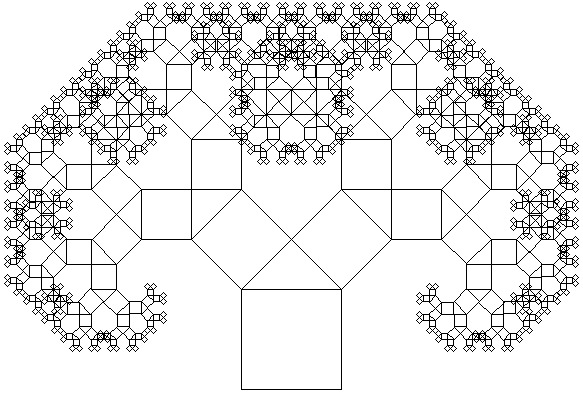
\includegraphics[scale = 0.5]{Classic.jpg}}
			\caption{Классическое дерево Пифагора}
			\label{ris:1}
		\end{center}
	\end{figure}

	\begin{figure}[h!]
		\begin{center}
			{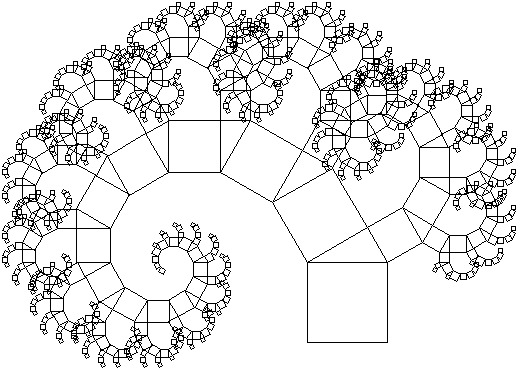
\includegraphics[scale = 0.5]{Wind.jpg}}
			\caption{Обдуваемое дерево Пифагора}
			\label{ris:2}
		\end{center}
	\end{figure}
	
	\begin{figure}[h!]
		\begin{center}
			{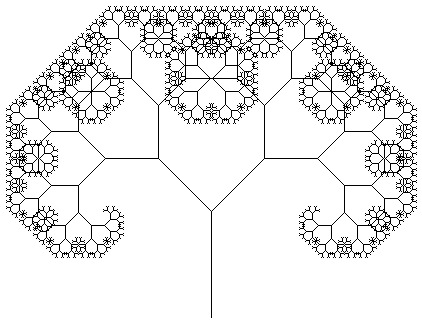
\includegraphics[scale = 0.5]{Neeked.jpg}}
			\caption{Обнаженное дерево Пифагора}
			\label{ris:3}
		\end{center}
	\end{figure}

	\newpage
	
	\subsection{Выводы}
	
	В рамках данного рубежного контроля было решено реализовать обнаженное дерево Пифагора в программе для курсового проекта по Компьютерной графике, так как она наилучшим образом подходит для реализации данного алгоритма.
	
	\section{Конструкторский раздел}
	
	Ниже представлен алгоритм построения дерева Пифагора:
	
	\begin{enumerate}
		\item Строим вертикальный отрезок
		\item Из верхнего конца этого отрезка рекурсивно строим еще 2 отрезка под определенными углами
		\item Вызываем функцию построения двух последующих отрезков для каждой ветви дерева
	\end{enumerate}
	
	\section{Технологический раздел}
	
	Здесь описываются требования к программному 
	обеспечению и средства реализации, приводятся листинги 
	программы и тестовые данные.
	
	\subsection{Требования к программному обеспечению}
	
	\begin{flushleft}
		\textbf{Входные данные:} 
		\begin{itemize}
			\item угол между ветками;
			\item толщина ветки;
			\item длина ветки.
		\end{itemize}
		\textbf{Выходные данные:} Массив точек, связанных между собой отрезками.
	\end{flushleft}

	\subsection{Средства реализации}
	
	Для реализации поставленной задачи был использован язык программирования C++ ~\cite{second}. Проет был выполнен в среде QT Creator ~\cite{third}. Для измерения процессорного времени была использована ассемблерная инструкция
	rdtsc ~\cite{fourth}.
	
	\subsection{Листинг программы}
	
	Реализованный алгоритм представлен
	в листинге \ref{lst1}.
	
	\begin{lstlisting}[label=lst1,caption=Реализация обнаженного дерева Пифагора]
		void model_nodes_fill(std::shared_ptr<Model> model, Binary_Tree *points)
		{
		Node node1(points->br.point1.x, points->br.point1.y, points->br.point1.z, {0, 0, 0});
		Node node2(points->br.point2.x, points->br.point2.y, points->br.point2.z, {0, 0, 0});
		
		model->addNode(node1);
		model->addNode(node2);
		
		if (points->left != nullptr)
		{
		model_nodes_fill(model, points->left);
		}
		
		if (points->right != nullptr)
		{
		model_nodes_fill(model, points->right);
		}
		}
		
		
		double calc_a_r(double a, double alpha)
		{
		return a * (sin(alpha) + cos(alpha) / 2);
		}
	
		double calc_pifagor_coord(double x, double a_r, double cos_alpha)
		{
		return x + a_r * cos_alpha;
		}
		
		void pifagor_algorithm_iter(Branch &br, Branch &next_br, double next_angle, double a, double alpha)
		{
		next_br.point1 = br.point2;
		double a_r = calc_a_r(a, alpha);
		
		double x = calc_pifagor_coord(next_br.point1.x, a_r, cos(next_angle));
		double y = calc_pifagor_coord(next_br.point1.y, a_r, sin(next_angle));
		next_br.point2.x = x;
		next_br.point2.y = y;
		next_br.point2.z = 0;
		}
		
		
		void create_next_pifagor_branch(Binary_Tree *tree, vector<double> &branch_radius, double next_angle, double alpha, size_t max_iteration, double a)
		{
		if (tree->br.depth == max_iteration)
		{
		return;
		}
		
		//double a = calc_length(tree->br.point1, tree->br.point2);
		
		tree->left = new Binary_Tree();
		tree->left->left = nullptr;
		tree->left->right = nullptr;
		
		tree->left->br.depth = tree->br.depth + 1;
		pifagor_algorithm_iter(tree->br, tree->left->br, M_PI / 2 + next_angle, a, M_PI / 2 - alpha);
		tree->left->br.radius = tree->br.radius / 1.1;
		branch_radius.push_back(tree->left->br.radius);
		
		create_next_pifagor_branch(tree->left, branch_radius, alpha + next_angle, alpha, max_iteration, cos(alpha) * a);
		
		tree->right = new Binary_Tree();
		tree->right->left = nullptr;
		tree->right->right = nullptr;
		
		tree->right->br.depth = tree->br.depth + 1;
		pifagor_algorithm_iter(tree->br, tree->right->br, next_angle, a, alpha);
		tree->right->br.radius = tree->br.radius / 1.1;
		branch_radius.push_back(tree->right->br.radius);
		create_next_pifagor_branch(tree->right, branch_radius, next_angle - (M_PI / 2 - alpha), alpha, max_iteration, sin(alpha) * a);
		
		}
		
		void pifagor_algorithm(Binary_Tree *tree, vector<double> &branch_radius, double a, double alpha, size_t iteration)
		{
		tree->br.depth = 0;
		tree->br.point1 = {0, 0, 0};
		tree->br.point2 = {0, a, 0};
		tree->br.radius = branch_radius[0];
		create_next_pifagor_branch(tree, branch_radius, alpha, alpha, iteration, a);
		}
		
		std::shared_ptr<Transformed_Model> Pifagor::buildModel(tree_params params, std::shared_ptr<Transform_Tree> tr_tree)
		{
		model = std::make_shared<Model>();
		
		double a = params.body.length;
		double alpha = params.angles.alpha1;
		
		size_t iteration = 11;
		
		size_t branches = get_tree_branches(iteration);
		
		size_t nodes_amount = branches * 2;
		
		vector<double> branch_radius;
		
		branch_radius.push_back(params.body.radius);
		
		Binary_Tree *nodes = new Binary_Tree();
		nodes->left = nullptr;
		nodes->right = nullptr;
		
		pifagor_algorithm(nodes, branch_radius, a, alpha, iteration);
		
		model_nodes_fill(this->model, nodes);
		
		edges_fill(this->model, nodes_amount, branch_radius);
		
		this->model->setAccuracy(params.body.accuracy);
		return tr_tree.get()->buildModel(model, params.tree_clr.clr);
		}
	\end{lstlisting}
	
	\section{Исследовательский раздел}
		
	В разделе представлены примеры выполнения программы.
	
	\subsection{Примеры работы}
	
	На рис. \ref{fig:t0}-\ref{fig:t4} приведены примеры работы программы. 
	
	\begin{figure}[h!]
		\center{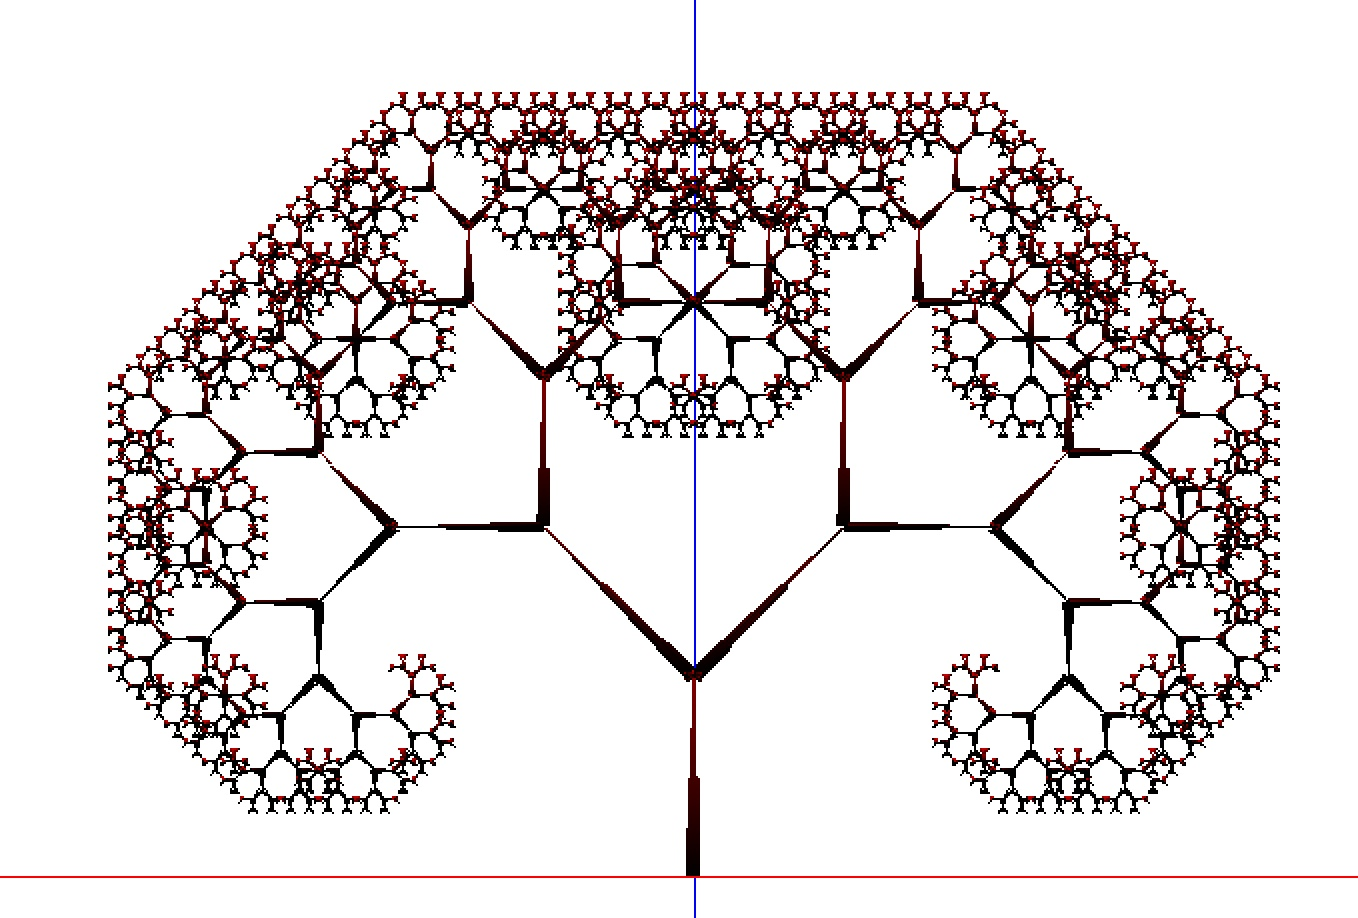
\includegraphics[scale = 0.25]{45.jpg}}
		\caption{
			Обнаженное классическое дерево Пифагора (Угол 45 градусов)}
		\label{fig:t0}
	\end{figure}

\newpage
	
	\begin{figure}[h!]
		\center{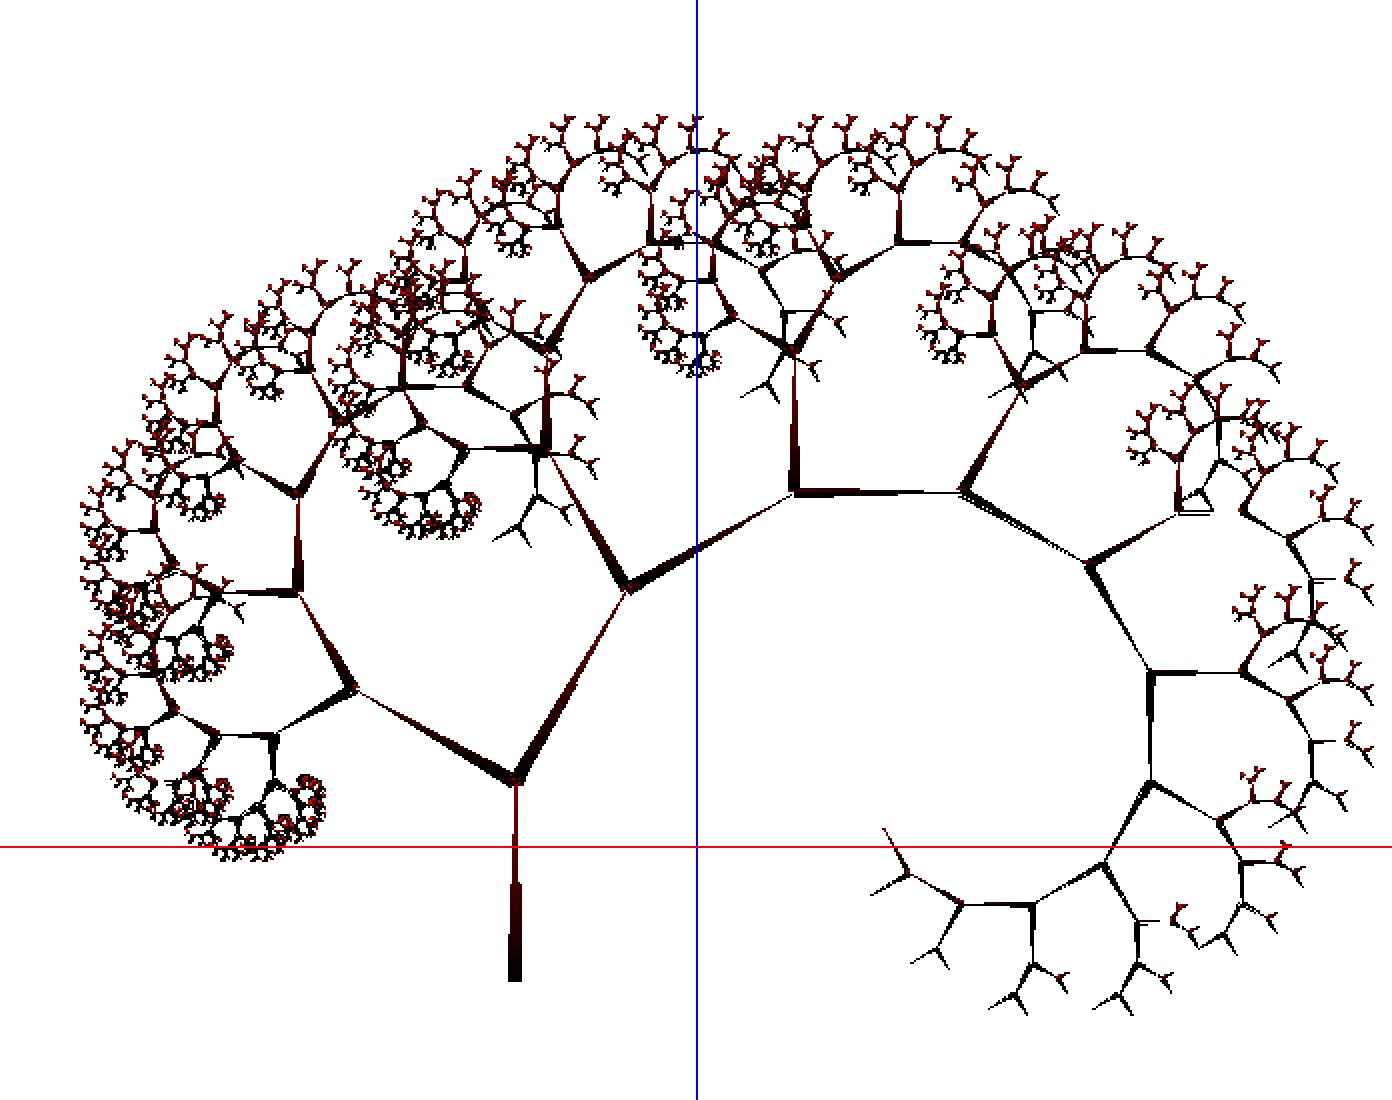
\includegraphics[scale = 0.25]{30.jpg}}
		\caption{
			Обнаженное обдуваемое дерево Пифагора (Угол 30 градусов)}
		\label{fig:t1}
	\end{figure}
	
	\begin{figure}[h!]
		\center{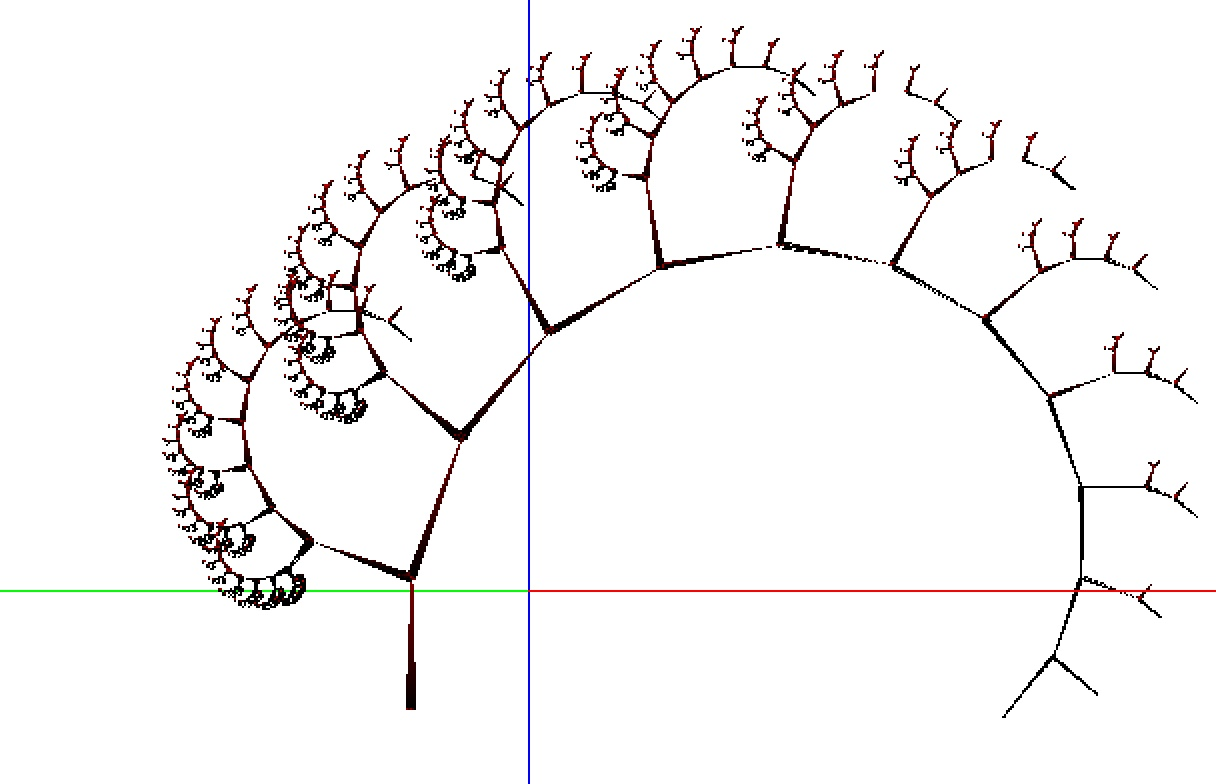
\includegraphics[scale = 0.25]{20.jpg}}
		\caption{
			Обнаженное обдуваемое дерево Пифагора (Угол 20 градусов)}
		\label{fig:t2}
	\end{figure}
	
\newpage
	
	\begin{figure}[h!]
		\center{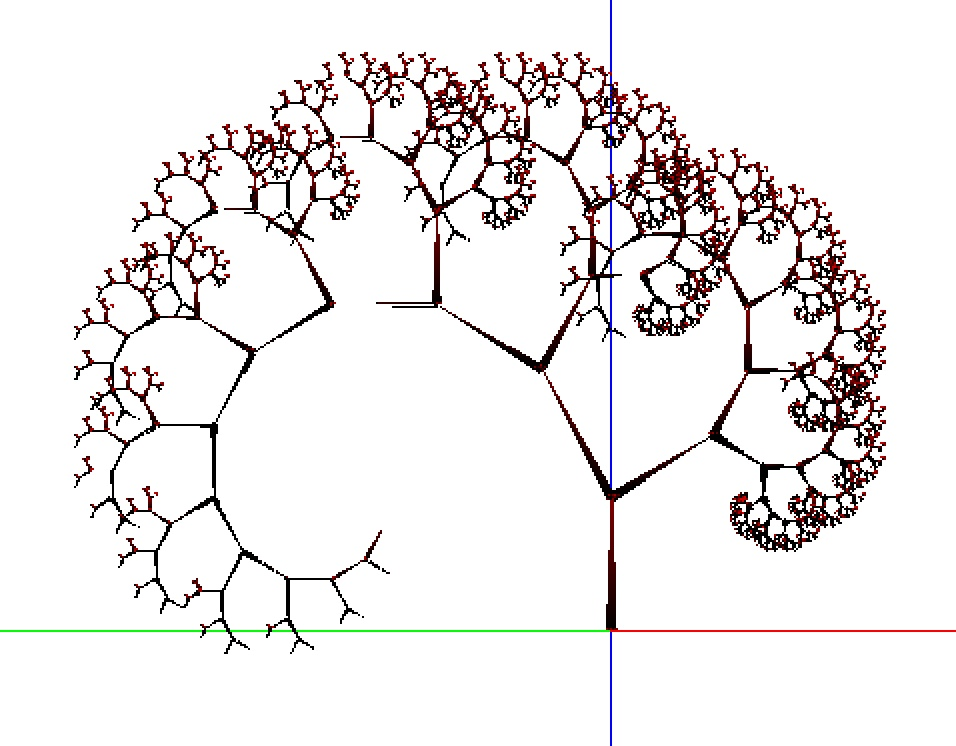
\includegraphics[scale = 0.25]{60.jpg}}
		\caption{
			Обнаженное обдуваемое дерево Пифагора (Угол 60 градусов)}
		\label{fig:t3}
	\end{figure}
	
	\begin{figure}[h!]
		\center{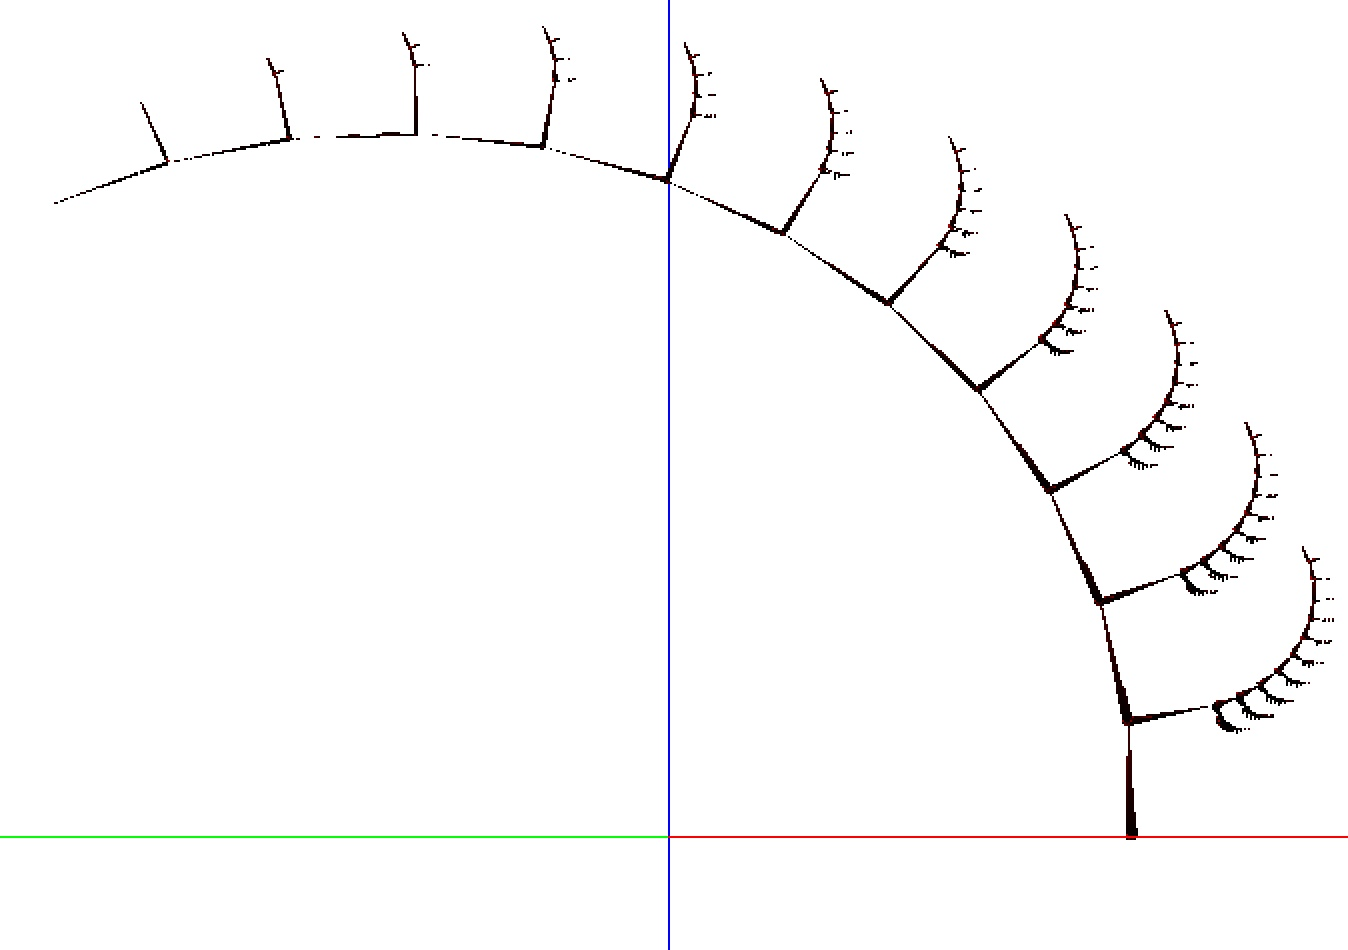
\includegraphics[scale = 0.25]{10.jpg}}
		\caption{
			Обнаженное обдуваемое дерево Пифагора (Угол 10 градусов)}
		\label{fig:t4}
	\end{figure}
		
		
	\section*{Заключение}
	\addcontentsline{toc}{section}{Заключение}
	
	~\
	
	В ходе выполнения данной лабораторной работы был изучен алгоритм построения фрактала дерева Пифагора. Алгоритм был разработан и реализацован.
	
	\newpage
	
	\addcontentsline{toc}{section}{Список литературы}
	\begin{thebibliography}{}
		
		\bibitem{second} ISO/IEC JTC1 SC22 WG21 N 3690 «Programming Languages — C++» [Электронный ресурс]. – Режим доступа: https://devdocs.io/cpp/, свободный. (Дата обращения: 29.09.2019 г.)
		
		\bibitem{third} QT Creator Manual [Электронный ресурс]. – Режим
		доступа: https://doc.qt.io/qtcreator/index.html, свободный. (Дата
		обращения: 29.09.2019 г.)
		
		\bibitem{fourth} Microsoft «rdtsc» [Электронный ресурс]. – Режим доступа:
		https://docs.microsoft.com/ru-ru/cpp/intrinsics/rdtsc?view=vs-2019,
		свободный. (Дата обращения: 29.09.2019 г.)
		
		\bibitem{tree}
		Pifagor algorithm [Электронный ресурс]. - Режим доступа:
		http://grafika.me/node/87 - (28.11.2019)
		
	\end{thebibliography}

\end{document}